% ==============================================================================
% Modelo para Monografia de Projeto de Graduação (PG)
% Prof. Vítor E. Silva Souza - Nemo / DI / UFES
%
% Baseado em abtex2-modelo-trabalho-academico.tex, v-1.9.2 laurocesar
% Copyright 2012-2014 by abnTeX2 group at http://abntex2.googlecode.com/ 
%
% This work may be distributed and/or modified under the conditions of the LaTeX 
% Project Public License, either version 1.3 of this license or (at your option) 
% any later version. The latest version of this license is in
% http://www.latex-project.org/lppl.txt.
%
% IMPORTANTE:
% Instruções encontram-se espalhadas pelo documento. Para facilitar sua leitura,
% tais instruções são precedidas por (*) -- utilize a função localizar do seu
% editor para passar por todas elas.
% ==============================================================================

% Usa o estilo abntex2, configurando detalhes de formatação e hifenização.
\documentclass[
	12pt,				% Tamanho da fonte.
	openright,			% Capítulos começam em página ímpar (insere página vazia caso preciso).
	oneside,			% Para impressão em verso e anverso. Oposto a oneside.
	a4paper,			% Tamanho do papel.
	english,			% Idioma adicional para hifenização.
	french,				% Idioma adicional para hifenização.
	spanish,			% Idioma adicional para hifenização.
	brazil				% O último idioma é o principal do documento.
	]{abntex2}



%%% Importação de pacotes. %%%
\usepackage{float}
\usepackage{adjustbox}
% Conserta o erro "No room for a new \count"
\usepackage{etex}
%\reserveinserts{28}

% Usa a fonte Latin Modern.
\usepackage{lmodern}

% Seleção de códigos de fonte.
\usepackage[T1]{fontenc}

% Codificação do documento em Unicode.
\usepackage[utf8]{inputenc}

% Usado pela ficha catalográfica.
\usepackage{lastpage}

% Indenta o primeiro parágrafo de cada seção.
\usepackage{indentfirst}

% Controle das cores.
\usepackage[usenames,dvipsnames]{xcolor}

% Inclusão de gráficos.
\usepackage{graphicx}

% Inclusão de páginas em PDF diretamente no documento (para uso nos apêndices).
\usepackage{pdfpages}

% Para melhorias de justificação.
\usepackage{microtype}

% Citações padrão ABNT.
\usepackage[brazilian,hyperpageref]{backref}
\usepackage[alf]{abntex2cite}	
\renewcommand{\backrefpagesname}{Citado na(s) página(s):~}		% Usado sem a opção hyperpageref de backref.
\renewcommand{\backref}{}										% Texto padrão antes do número das páginas.
\renewcommand*{\backrefalt}[4]{									% Define os textos da citação.
	\ifcase #1
		Nenhuma citação no texto.
	\or
		Citado na página #2.
	\else
		Citado #1 vezes nas páginas #2.
	\fi}

% \rm is deprecated and should not be used in a LaTeX2e document
% http://tex.stackexchange.com/questions/151897/always-textrm-never-rm-a-counterexample
\renewcommand{\rm}{\textrm}

% Pacotes não incluídos no template abntex2. 
% Podem ser comentados caso não queira utilizá-los.

% Inclusão de símbolos não padrão.
\usepackage{amssymb}
\usepackage{eurosym}

% Para utilizar \eqref para referenciar equações.
\usepackage{amsmath}

% Permite mostrar figuras muito largas em modo paisagem com \begin{sidewaysfigure} ao invés de \begin{figure}.
\usepackage{rotating}

% Permite customizar listas enumeradas/com marcadores.
\usepackage{enumitem}

% Permite inserir hiperlinks com \url{}.
\usepackage{bigfoot}
\usepackage{hyperref}

% Permite usar o comando \hl{} para evidenciar texto com fundo amarelo. Útil para chamar atenção a itens a fazer.
\usepackage{soulutf8}

% Colorinlistoftodos package: to insert colored comments so authors can collaborate on the content.
\usepackage[colorinlistoftodos, textwidth=20mm, textsize=footnotesize]{todonotes}
\newcommand{\aluno}[1]{\todo[author=\textbf{Aluno},color=green!30,caption={},inline]{#1}}
\newcommand{\professor}[1]{\todo[author=\textbf{Professor},color=red!30,caption={},inline]{#1}}

% Permite inserir espaço em branco condicional (incluído no texto final só se necessário) em macros.
\usepackage{xspace}

% Permite incluir listagens de código com o comando \lstinputlisting{}.
\usepackage{listings}
\usepackage{caption}
\DeclareCaptionFont{white}{\color{white}}
\DeclareCaptionFormat{listing}{\colorbox{gray}{\parbox{\textwidth}{#1#2#3}}}
\captionsetup[lstlisting]{format=listing,labelfont=white,textfont=white}
\renewcommand{\lstlistingname}{Listagem}
\definecolor{mygray}{rgb}{0.5,0.5,0.5}
\lstset{
	basicstyle=\scriptsize,
	breaklines=true,
	numbers=left,
	numbersep=5pt,
	numberstyle=\tiny\color{mygray}, 
	rulecolor=\color{black},
	showstringspaces=false,
	tabsize=2,
    inputencoding=utf8,
    extendedchars=true,
    literate=%
    {é}{{\'{e}}}1
    {è}{{\`{e}}}1
    {ê}{{\^{e}}}1
    {ë}{{\¨{e}}}1
    {É}{{\'{E}}}1
    {Ê}{{\^{E}}}1
    {û}{{\^{u}}}1
    {ù}{{\`{u}}}1
    {â}{{\^{a}}}1
    {à}{{\`{a}}}1
    {á}{{\'{a}}}1
    {ã}{{\~{a}}}1
    {Á}{{\'{A}}}1
    {Â}{{\^{A}}}1
    {Ã}{{\~{A}}}1
    {ç}{{\c{c}}}1
    {Ç}{{\c{C}}}1
    {õ}{{\~{o}}}1
    {ó}{{\'{o}}}1
    {ô}{{\^{o}}}1
    {Õ}{{\~{O}}}1
    {Ó}{{\'{O}}}1
    {Ô}{{\^{O}}}1
    {î}{{\^{i}}}1
    {Î}{{\^{I}}}1
    {í}{{\'{i}}}1
    {Í}{{\~{Í}}}1
}



%%% Definição de variáveis. %%%

% (*) Substituir os textos abaixo com as informações apropriadas.
\titulo{Estudo sobre Algoritmos de Menor Caminho em Grafos}
\autor{Pedro}
\local{Vitória, ES}
\data{2017}
\orientador{Prof. Dra. Maria Cláudia Silva Boeres}
%\coorientador{Nome do Co-orientador}
\instituicao{
  Universidade Federal do Espírito Santo -- UFES
  \par
  Centro Tecnológico
  \par
  Departamento de Informática}
\tipotrabalho{Monografia (PG)}

% Preâmbulo (tipo do trabalho, objetivo, nome da instituição, área de concentração, etc.).
% (*) Verificar se está correto (ex.: substituir por Engenharia de Computação se for o caso).
\preambulo{Monografia apresentada ao Curso de Ciência da Computação do Departamento de Informática da Universidade Federal do Espírito Santo, como requisito parcial para obtenção do Grau de Bacharel em Ciência da Computação.}

% Macros específicas do trabalho.
% (*) Inclua aqui termos que são utilizados muitas vezes e que demandam formatação especial.
% Os exemplos abaixo incluem i* (substituindo o asterisco por uma estrela) e Java com TM em superscript.
% Use sempre \xspace para que o LaTeX inclua espaço em branco após a macro somente quando necessário.
\newcommand{\istar}{\textit{i}$^\star$\xspace}
\newcommand{\java}{Java\texttrademark\xspace}
\newcommand{\latex}{\LaTeX\xspace}




%%% Configurações finais de aparência. %%%

% Altera o aspecto da cor azul.
\definecolor{blue}{RGB}{41,5,195}

% Informações do PDF.
\makeatletter
\hypersetup{
	pdftitle={\@title}, 
	pdfauthor={\@author},
	pdfsubject={\imprimirpreambulo},
	pdfcreator={LaTeX with abnTeX2},
	pdfkeywords={abnt}{latex}{abntex}{abntex2}{trabalho acadêmico}, 
	colorlinks=true,				% Colore os links (ao invés de usar caixas).
	linkcolor=blue,					% Cor dos links.
	citecolor=blue,					% Cor dos links na bibliografia.
	filecolor=magenta,				% Cor dos links de arquivo.
	urlcolor=blue,					% Cor das URLs.
	bookmarksdepth=4
}
\makeatother

% Espaçamentos entre linhas e parágrafos.
\setlength{\parindent}{1.3cm}
\setlength{\parskip}{0.2cm}



%%% Páginas iniciais do documento: capa, folha de rosto, ficha, resumo, tabelas, etc. %%%

% Compila o índice.
\makeindex

% Inicia o documento.
\begin{document}

% Retira espaço extra obsoleto entre as frases.
\frenchspacing

% Capa do trabalho.
\imprimircapa

% Folha de rosto (o * indica que haverá a ficha bibliográfica).
\imprimirfolhaderosto*


% Ficha catalográfica.
% (*) Escolher entre as versões de ficha catalográfica abaixo (comente aquela que não quiser usar).

% Versão 1: caso a biblioteca da sua universidade lhe forneça um PDF (adequar o nome do arquivo).
% \begin{fichacatalografica}
%     \includepdf{include-fichacatalografica.pdf}
% \end{fichacatalografica}

% Versão 2: caso você tenha que inserir sua própria ficha catalográfica.
% (*) Neste caso, preencher palavras-chave e adicione co-orientador (se houver).
\begin{fichacatalografica}
	\vspace*{\fill}
	\hrule
	\begin{center}
	\begin{minipage}[c]{12.5cm}
	
	\imprimirautor
	
	\hspace{0.5cm} \imprimirtitulo  / \imprimirautor. --
	\imprimirlocal, \imprimirdata-
	
	\hspace{0.5cm} \pageref{LastPage} p. : il. (algumas color.) ; 30 cm.\\
	
	\hspace{0.5cm} \imprimirorientadorRotulo~\imprimirorientador\\
	
	\hspace{0.5cm}
	\parbox[t]{\textwidth}{\imprimirtipotrabalho~--~\imprimirinstituicao,
	\imprimirdata.}\\
	
	\hspace{0.5cm}
		1. Palavra-chave1.
		2. Palavra-chave2.
		I. Souza, Vítor Estêvão Silva.
		II. Universidade Federal do Espírito Santo.
		IV. \imprimirtitulo \\ 			
	
	\hspace{8.75cm} CDU 02:141:005.7\\
	
	\end{minipage}
	\end{center}
	\hrule
\end{fichacatalografica}


% Folha de aprovação.
% (*) Escolher entre as versões de ficha catalográfica abaixo (comente aquela que não quiser usar).

% Versão 1: cópia digitalizada da folha de aprovação assinada pela banca.
% \includepdf{include-folhadeaprovacao.pdf}

% Versão 2: folha de aprovação em branco.
% (*) Ajustar a data e os nomes dos participantes da banca.
\begin{folhadeaprovacao}
  \begin{center}
    {\ABNTEXchapterfont\large\imprimirautor}
    \vspace*{\fill}\vspace*{\fill}
    \begin{center}
      \ABNTEXchapterfont\bfseries\Large\imprimirtitulo
    \end{center}
    \vspace*{\fill}
    \hspace{.45\textwidth}
    \begin{minipage}{.5\textwidth}
        \imprimirpreambulo
    \end{minipage}%
    \vspace*{\fill}
   \end{center}
   Trabalho aprovado. \imprimirlocal, 25 de setembro de 2017:
   \assinatura{\textbf{\imprimirorientador} \\ Orientador} 
   \assinatura{\textbf{Professor} \\ Convidado 1}
   \assinatura{\textbf{Professor} \\ Convidado 2}
   %\assinatura{\textbf{Professor} \\ Convidado 3}
   %\assinatura{\textbf{Professor} \\ Convidado 4}
   \begin{center}
    \vspace*{0.5cm}
    {\large\imprimirlocal}
    \par
    {\large\imprimirdata}
    \vspace*{1cm}
  \end{center}  
\end{folhadeaprovacao}


% Dedicatória.
% (*) Escrever dedicatória ou remover/comentar seção.
\begin{dedicatoria}
   \vspace*{\fill}
   \centering
   \noindent
   \textit{Lorem ipsum dolor sit amet, consectetur adipiscing elit. Duis malesuada laoreet leo at interdum. Nullam neque eros, dignissim sed ipsum sed, sagittis laoreet nisi.} \vspace*{\fill}
\end{dedicatoria}


% Agradecimentos.
% (*) Escrever agradecimentos ou remover/comentar seção.
\begin{agradecimentos}
Lorem ipsum dolor sit amet, consectetur adipiscing elit. Duis malesuada laoreet leo at interdum. Nullam neque eros, dignissim sed ipsum sed, sagittis laoreet nisi. Duis a pulvinar nisl. Aenean varius nisl eu magna facilisis porttitor. Cum sociis natoque penatibus et magnis dis parturient montes, nascetur ridiculus mus. Ut mattis tortor nisi, facilisis molestie arcu hendrerit sed. Donec placerat velit at odio dignissim luctus. Suspendisse potenti. Integer tristique mattis arcu, ut venenatis nulla tempor non. Donec at tincidunt nulla. Cras ac dignissim neque. Morbi in odio nulla. Donec posuere sem finibus, auctor nisl eu, posuere nisl. Duis sit amet neque id massa vehicula commodo dapibus eu elit. Sed nec leo eu sem viverra aliquet. Nam at nunc nec massa rutrum aliquam sed ac ante.

Vivamus nec quam iaculis, tempus ipsum eu, cursus ante. Phasellus cursus euismod auctor. Fusce luctus mauris id tortor cursus, volutpat cursus lacus ornare. Proin tristique metus sed est semper, id finibus neque efficitur. Cras venenatis augue ac venenatis mollis. Maecenas nec tellus quis libero consequat suscipit. Aliquam enim leo, pretium non elementum sit amet, vestibulum ut diam. Maecenas vitae diam ligula.

Fusce ac pretium leo, in convallis augue. Mauris pulvinar elit rhoncus velit auctor finibus. Praesent et commodo est, eu luctus arcu. Vivamus ut porta tortor, eget facilisis ex. Nunc aliquet tristique mauris id sollicitudin. Donec quis commodo metus, sit amet accumsan nibh. Cum sociis natoque penatibus et magnis dis parturient montes, nascetur ridiculus mus.
\end{agradecimentos}


% Epígrafe.
% (*) Escrever epígrafe ou remover/comentar seção.
\begin{epigrafe}
    \vspace*{\fill}
	\begin{flushright}
		\textit{``Lorem ipsum dolor sit amet, consectetur adipiscing elit. \\
		Duis malesuada laoreet leo at interdum. Nullam neque eros, dignissim \\
		sed ipsum sed, sagittis laoreet nisi.\\
		(Lipsum generator)}
	\end{flushright}
\end{epigrafe}


% Resumo em português.
% (*) Escrever resumo e palavras-chave.
\setlength{\absparsep}{18pt}
\begin{resumo}
Lorem ipsum dolor sit amet, consectetur adipiscing elit. Duis malesuada laoreet leo at interdum. Nullam neque eros, dignissim sed ipsum sed, sagittis laoreet nisi. Duis a pulvinar nisl. Aenean varius nisl eu magna facilisis porttitor. Cum sociis natoque penatibus et magnis dis parturient montes, nascetur ridiculus mus. Ut mattis tortor nisi, facilisis molestie arcu hendrerit sed. Donec placerat velit at odio dignissim luctus. Suspendisse potenti. Integer tristique mattis arcu, ut venenatis nulla tempor non. Donec at tincidunt nulla. Cras ac dignissim neque. Morbi in odio nulla. Donec posuere sem finibus, auctor nisl eu, posuere nisl. Duis sit amet neque id massa vehicula commodo dapibus eu elit. Sed nec leo eu sem viverra aliquet. Nam at nunc nec massa rutrum aliquam sed ac ante.

Vivamus nec quam iaculis, tempus ipsum eu, cursus ante. Phasellus cursus euismod auctor. Fusce luctus mauris id tortor cursus, volutpat cursus lacus ornare. Proin tristique metus sed est semper, id finibus neque efficitur. Cras venenatis augue ac venenatis mollis. Maecenas nec tellus quis libero consequat suscipit. Aliquam enim leo, pretium non elementum sit amet, vestibulum ut diam. Maecenas vitae diam ligula.

Fusce ac pretium leo, in convallis augue. Mauris pulvinar elit rhoncus velit auctor finibus. Praesent et commodo est, eu luctus arcu. Vivamus ut porta tortor, eget facilisis ex. Nunc aliquet tristique mauris id sollicitudin. Donec quis commodo metus, sit amet accumsan nibh. Cum sociis natoque penatibus et magnis dis parturient montes, nascetur ridiculus mus.

Duis elementum dictum tristique. Integer mattis libero sit amet pretium euismod. Curabitur auctor eu augue ut ornare. Integer bibendum eros ullamcorper rhoncus convallis. Pellentesque non pretium ligula, sit amet bibendum eros. Nam venenatis ex felis, quis blandit nunc auctor sit amet. Maecenas ut eros pharetra, lobortis neque id, fermentum arcu. Cras neque dui, rhoncus feugiat leo id, semper facilisis lorem. Fusce non ex turpis. Nullam venenatis sed ligula ac lacinia.

\textbf{Palavras-chaves}: lorem. ipsum. dolor. sit. amet.
\end{resumo}

% Insere lista de ilustrações.
\pdfbookmark[0]{\listfigurename}{lof}
\listoffigures*
\cleardoublepage

% Insere lista de tabelas.
\pdfbookmark[0]{\listtablename}{lot}
\listoftables*
\cleardoublepage

% Lista de abreviaturas e siglas.
% (*) Preencher com as siglas usadas ao longo do texto e seus significados.
\begin{siglas}
  \item[UML] Unified Modeling Language
\end{siglas}

% Insere o sumário.
\pdfbookmark[0]{\contentsname}{toc}
\tableofcontents*
\cleardoublepage



%%% Início da parte de conteúdo do documento. %%%

% Marca o início dos elementos textuais.
\textual

% Inclusão dos capítulos.
% (*) Para facilitar a organização, os capítulos foram divididos em arquivo separados e colocados dentro da.
% pasta capitulos/. Caso o aluno prefira trabalhar com um só arquivo, basta substituir os comandos \include 
% pelos conteúdos dos arquivos que estão sendo incluídos, excluindo a pasta capitulos/ em seguida.
% ==============================================================================
% TCC - Nome do Aluno
% Capítulo 1 - Introdução
% ==============================================================================
\chapter{Introdução}
\label{sec-intro}
Na computação muitas aplicações necessitam considerar um conjunto um conjunto de conexões entre dados e uso de algoritmos nesses dados para poder responder perguntad como, se existe um caminho entre um objeto a outro seguindo por essas conexões, qual a menor dinstância entre eles ou ainda quantos objetos podemos alcançar a partir de um determinado ponto. Para modelar tais situações, utilizamos um tipo abstrato chamado grafo \cite{ziviani2004projeto}.

Um problema clássico da literatura envolvendo grafos é o cálculo de caminho mínimo \cite{moura2010estudo}. Nele desejamos obter o menor caminho entre dois pontos específicos do grafo representado. A sua modelagem é feita representando as arestas com determinados pesos que podem significar o tempo decorrente entre executar tarefas, o custo de transmitir informações entre locais, quantidades específicas a serem transportadas entre um local e outro e etc \cite{drozdek2012data}. 

Dentre as modelagens realizadas para resolver o problema do caminho mínimo, uma que é abordada é a definição do menor caminho entre dois pontos geográficos tendo como aplicação prática o uso por softwares do tipo GPS. Nela representamos as interseções das ruas, caminhos ou rodovias como o vértices do grafo e as distâncias entre essas interseções (as próprias ruas, caminhos ou rodovias) como as arestas e tendo seus respectivos pesos como sendo a distâncias entre essas interseções.

A figura X mostra o exemplo desta modelagem abordada.

A motivação deste trabalho é o estudo dos algoritmos de menor caminho em grafos, desde os clássicos como o algoritmo de Dijkstra \cite{dijkstra1959note} até algoritmos mais recentes propostos como o Anytime Dynamic A* (AD*) \cite{likhachev2008anytime}. Tem por  objetivo verificar o desempenho e a eficácia destes algoritmos, averiguar o impacto que as estruturas de dados utilizadas para resolver o problema causam e analisar quais situações os algoritmos estudados melhor se aplicam.

\section{Objetivos}
\label{sec-intro-objetivos}

\section{Organização dos capítulos}
\label{sec-intro-organizaocao}

%%% Início de seção. %%%
\section{Seções e subseções}
\label{sec-intro-secoes}

O documento é organizado em capítulos (\texttt{\textbackslash chapter\{\}}), seções (\texttt{\textbackslash section\{\}}), subseções (\texttt{\textbackslash subsection\{\}}), sub-subseções (\texttt{\textbackslash subsubsection\{\}}) e assim por diante. Atenção, porém, a não criar estruturas muito profundas (sub-sub-sub-...) pois o documento não fica bem estruturado.


%%% Início de seção. %%%
\subsection{Referências a seções}
\label{sec-intro-secoes-refs}

Cada parte do documento (capítulo, seção, etc.) deve possuir um rótulo logo abaixo de sua definição. Por exemplo, este capítulo é definido com \texttt{\textbackslash chapter\{Introdução\}} seguido por \texttt{\textbackslash label\{sec-intro\}}. Assim, podemos fazer referências cruzadas usando o comando \texttt{\textbackslash ref\{rótulo\}}: ``O Capítulo~\ref{sec-intro} começa com a Seção~\ref{sec-intro-secoes}, que é ainda subdividida nas subseções~\ref{sec-intro-secoes-refs} e~\ref{sec-intro-secoes-sobrerefs}.

Para melhor organização das partes do documento, sugere-se primeiro utilizar o prefixo \texttt{sec-} (para diferenciar de referências à figuras, tabelas, etc. quando usarmos o comando \texttt{\textbackslash ref\{\}}) e também representar a hierarquia das seções nos rótulos. Por exemplo, o Capítulo~\ref{sec-intro} tem rótulo \texttt{sec-intro}, sua Seção~\ref{sec-intro-secoes} tem rótulo \texttt{sec-intro-secoes} e a Subseção~\ref{sec-intro-secoes-refs} tem rótulo \texttt{sec-intro-secoes-refs}.



%%% Início de seção. %%%
\subsection{Sobre referências cruzadas}
\label{sec-intro-secoes-sobrerefs}

Nas próximas seções, veremos que é possível fazer referência cruzada não só a seções mas também a listagens de código, figuras, tabelas, etc. Em todos estes casos, quando nos referimos à Seção X, Listagem Y ou Figura Z, consideramos que estes são os nomes próprios destes elementos e, portanto, usa-se a primeira letra maiúscula. Isso pode ser visto na Subseção~\ref{sec-intro-secoes-refs}, acima. A exceção é quando nos referimos a vários elementos ao mesmo tempo, por exemplo: ``as subseções~\ref{sec-intro-secoes-refs} e~\ref{sec-intro-secoes-sobrerefs}''.

Por fim, ao usar o comando \texttt{\textbackslash ref\{\}}, sugere-se separá-lo da palavra que vem antes dele com um \textasciitilde\ ao invés de espaço. Por exemplo: \texttt{o capítulo\textasciitilde \textbackslash ref\{sec-intro\}}. Isso faz com que o \latex não quebre linha entre a palavra \texttt{capítulo} e o número do capítulo.




%%% Início de seção. %%%
\section{Citações bibliográficas}
\label{sec-intro-citacoes}

Este documento utiliza a ferramenta de gerenciamento de referências bibliográficas do \latex, chamada \emph{BibTeX}. O arquivo \texttt{bibliografia.bib}, referenciado no arquivo \latex principal deste documento, contém algumas referências bibliográficas de exemplo. Assim como capítulos, seções, etc., tais referências também possuem rótulos, especificados como primeiro parâmetro de cada entrada (ex.: \texttt{@incollection\{souza-et-al:iism08, ...\}}.

Sugere-se um padrão para rótulos de referências bibliográficas para que fique claro também no código \latex qual referência está sendo citada. Por exemplo, ao citar a referência \texttt{souza-et-al:sesas13}, sabemos que é um artigo escrito por \emph{Souza} e outros, publicado no \emph{SESAS} em \emph{2013} (geralmente a pessoa que citou sabe que publicação é SESAS e quem é Souza).

Para citar uma referência bibliográfica contida no arquivo \emph{BibTeX}, basta usar seu rótulo como parâmetro de um de dois comandos possíveis de citação:

\begin{itemize}
\item O comando \texttt{\textbackslash cite\{\}} efetua uma citação tradicional, colocando o nome do(s) autor(es) e o ano entre parênteses. Por exemplo, \texttt{\textbackslash cite\{souza-et-al:iism08\}} é transformado em \cite{souza-et-al:iism08};

\item O comando \texttt{\textbackslash citeonline\{\}} efetua uma citação integrada ao texto, colocando o nome do(s) autor(es) direto no texto e somente o ano entre parênteses. Por exemplo, ``de acordo com \texttt{\textbackslash citeonline\{souza-et-al:iism08\}}'' é transformado em: de acordo com \citeonline{souza-et-al:iism08};
\end{itemize}

Também é possível citar vários trabalhos de uma só vez, separando os rótulos das referências bibliográficas com uma vírgula dentro do comando apropriado. Por exemplo, \texttt{\textbackslash cite\{souza-et-al:sesas13,souza-et-al:csrd13\}} \cite{souza-et-al:sesas13,souza-et-al:csrd13}.

Os trabalhos citados são automaticamente incluídos na seção de referências bibliográficas, ao final do documento. Tudo é formatado automaticamente segundo padrões da ABNT.



%%% Início de seção. %%%
\section{Listagens de código}
\label{sec-intro-listagens}

O pacote \texttt{listings}, incluído neste template, permite a inclusão de listagens de código. Análogo ao já feito anteriormente, listagens possuem rótulos para que possam ser referenciadas e sugerimos uma regra de nomenclatura para tais rótulos: usar como prefixo o rótulo do capítulo, substituindo \texttt{sec-} por \texttt{lst-}.

A Listagem~\ref{lst-intro-exemplo}, por exemplo, possui o rótulo \texttt{lst-intro-exemplo} e representa o código que foi usado no próprio documento para exibir as listagens desta seção. Como podemos ver, a sugestão é que os arquivos de código sejam colocados dentro da pasta \texttt{codigos/} e tenham nome idêntico ao rótulo, colocando a extensão adequada ao tipo de código.

\lstinputlisting[label=lst-intro-exemplo, caption=Exemplo de código \latex para inclusão de listagens de código., float=htpb]{codigos/lst-intro-exemplo.tex}

A Listagem~\ref{lst-intro-outroexemplo} mostra um exemplo de listagem com especificação da linguagem utilizada no código. O pacote \texttt{listings} reconhece algumas linguagens\footnote{Veja a lista de linguagens suportadas em \url{http://en.wikibooks.org/wiki/LaTeX/Source\_Code\_Listings\#Supported_languages}.} e faz ``coloração'' de código (na verdade, usa \textbf{negrito} e não cores) de acordo com a linguagem. O parâmetro \texttt{float=htpb} incluído em ambos os exemplos impede que a listagem seja quebrada em diferentes páginas.

\lstinputlisting[label=lst-intro-outroexemplo, caption=Exemplo de código \java especificando linguagem utilizada., language=Java, float=htpb]{codigos/lst-intro-outroexemplo.java}



%%% Início de seção. %%%
\section{Figuras}
\label{sec-intro-figuras}

Figuras podem ser inseridas no documento usando o \emph{ambiente} \texttt{figure} (ou seja, \texttt{\textbackslash begin\{figure\}} e \texttt{\textbackslash end\{figure\}}) e o comando \texttt{\textbackslash includegraphics\{\}}. Existem alguns outros elementos e propriedades úteis de serem configuradas, resultando no código exibido na Listagem~\ref{lst-intro-figuras}.

\lstinputlisting[label=lst-intro-figuras, caption=Código \latex utilizado para inclusão das figuras na Seção~\ref{sec-intro-figuras}., float=htpb]{codigos/lst-intro-figuras.tex}

O comando \texttt{\textbackslash centering} centraliza a figura na página. A opção \texttt{width} do comando \texttt{\textbackslash includegraphics\{\}} determina o tamanho da figura e usa-se \texttt{\textbackslash textwidth} (opcionalmente multiplicado por um número) para se referir à largura da página.

O parâmetro do comando \texttt{\textbackslash includegraphics\{\}} indica onde a imagem pode ser encontrada. Foi criado o diretório \texttt{figuras/} para conter as figuras do documento, dando uma melhor organização aos arquivos. Ao abrir esta pasta, repare que as figuras possuem duas versões---uma em \texttt{.eps} e outra em \texttt{.pdf}---e que o comando \texttt{\textbackslash includegraphics\{\}} não especifica a extensão. Isso se dá porque o \latex possui um compilador para formato PostScript (\texttt{latex}) que espera as imagens em \texttt{.eps} e um compilador para PDF (\texttt{pdflatex}) que espera as imagens em \texttt{.pdf}.

Por fim, o comando \texttt{\textbackslash caption\{\}} especifica a descrição da figura e \texttt{\textbackslash label\{\}}, como de costume, estabelece um rótulo para permitir referência cruzada de figuras. Note ainda que é utilizada a mesma estratégia de nomenclatura de rótulos usada nas listagens, porém utilizando o prefixo \texttt{fig-}.

As figuras~\ref{fig-intro-nemologo} e~\ref{fig-intro-exemplosideways} mostram o resultado do código da Listagem~\ref{lst-intro-figuras}. A Figura~\ref{fig-intro-exemplosideways}, em particular, utiliza o pacote \texttt{rotating} para mostrar figuras largas em modo paisagem. Basta usar o ambiente \texttt{sidewaysfigure} ao invés de \texttt{figure}.

\begin{figure}
\centering

\includegraphics[width=.25\textwidth]{figuras/fig-intro-nemologo} 
\caption{Exemplo de figura: logo do Nemo.}
\label{fig-intro-nemologo}
\end{figure}

\begin{sidewaysfigure}
\centering
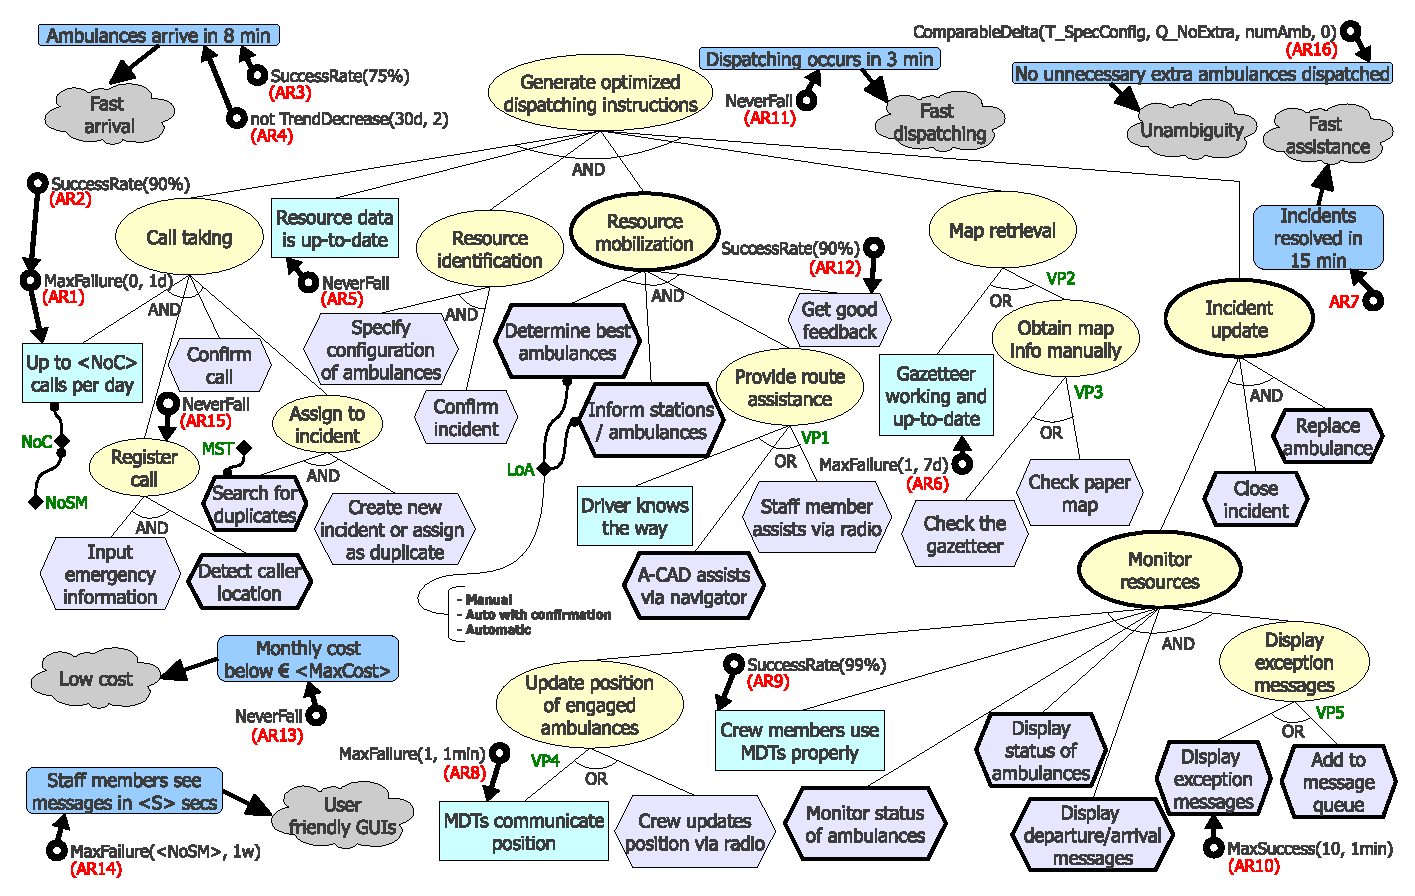
\includegraphics[width=\textwidth]{figuras/fig-intro-exemplosideways} 
\caption{Exemplo de figura em modo paisagem: um modelo de objetivos~\cite{souza-mylopoulos:spe13}.}
\label{fig-intro-exemplosideways}
\end{sidewaysfigure}



%%% Início de seção. %%%
\section{Tabelas}
\label{sec-intro-tabelas}

Tabelas são um ponto fraco do \latex. Elas são complicadas de fazer e, dependendo da complexidade da tabela (muitas células mescladas, por exemplo), vale a pena construi-las em outro programa (por exemplo, em seu editor de texto favorito), converter para PDF e inclui-las no documento como figuras. Mostramos, no entanto, alguns exemplos de tabela a seguir. O código utilizado para criar as tabelas encontra-se nas listagens~\ref{lst-intro-tabelas01} e~\ref{lst-intro-tabelas02}. 

\lstinputlisting[label=lst-intro-tabelas01, caption=Código \latex utilizado para inclusão das tabelas~\ref{tbl-intro-exemplo01} e~\ref{tbl-intro-exemplo02}., float=htpb]{codigos/lst-intro-tabelas01.tex}

\lstinputlisting[label=lst-intro-tabelas02, caption=Código \latex utilizado para inclusão da Tabela~\ref{tbl-intro-exemplo03}., float=htpb]{codigos/lst-intro-tabelas02.tex}

% Exemplo de tabela 01:
\begin{table}
\caption{Exemplo de tabela com diferentes alinhamentos de conteúdo.}
\label{tbl-intro-exemplo01}
\centering
\begin{tabular}{ | c | l | r | p{40mm} |}\hline
\textbf{Centralizado} & \textbf{Esquerda} & \textbf{Direita} & \textbf{Parágrafo}\\\hline
C & L & R & Alinhamento de tipo parágrafo especifica largura da coluna e quebra o texto automaticamente.\\
\hline
Linha 2 & Linha 2 & Linha 2 & Linha 2\\
\hline
\end{tabular}
\end{table}

% Exemplo de tabela 02:
\begin{table}
\caption{Exemplo que especifica largura de coluna e usa lista enumerada (adaptada de~\cite{souza-mylopoulos:spe13}).}
\label{tbl-intro-exemplo02}
\centering
\renewcommand{\arraystretch}{1.2}
\begin{small}
\begin{tabular}{ | p{15mm} | p{77mm} | p{55mm} |}\hline
\textbf{\textit{AwReq}} & \textbf{Adaptation strategies} & \textbf{Applicability conditions}\\\hline

AR1 &
\vspace{-2mm}\begin{enumerate}[topsep=0cm, partopsep=0cm, itemsep=0cm, parsep=0cm, leftmargin=0.5cm]
\item \textit{Warning(``AS Management'')}
\item \textit{Reconfigure($\varnothing$)}
\end{enumerate}\vspace{-4mm} &
\vspace{-2mm}\begin{enumerate}[topsep=0cm, partopsep=0cm, itemsep=0cm, parsep=0cm, leftmargin=0.5cm]
\item Once per adaptation session;
\item Always.
\end{enumerate}\vspace{-4mm}
\\\hline

AR2 &
\vspace{-2mm}\begin{enumerate}[topsep=0cm, partopsep=0cm, itemsep=0cm, parsep=0cm, leftmargin=0.5cm]
\item \textit{Warning(``AS Management'')}
\item \textit{Reconfigure($\varnothing$)}
\end{enumerate}\vspace{-4mm} &
\vspace{-2mm}\begin{enumerate}[topsep=0cm, partopsep=0cm, itemsep=0cm, parsep=0cm, leftmargin=0.5cm]
\item Once per adaptation session;
\item Always.
\end{enumerate}\vspace{-4mm}
\\\hline
\end{tabular}
\end{small}
\end{table}

% Exemplo de tabela 03:
\begin{table}
\caption{Exemplo que mostra equações em duas colunas (adaptada de~\cite{souza-mylopoulos:spe13}).}
\label{tbl-intro-exemplo03}
\centering
\vspace{1mm}
\fbox{\begin{minipage}{.98\linewidth}
\begin{minipage}{0.51\linewidth}
\vspace{-4mm}
\begin{eqnarray}
\Delta \left( I_{AR1} / NoSM \right) \left[ 0, maxSM \right] > 0\\
\Delta \left( I_{AR2} / NoSM \right) \left[ 0, maxSM \right] > 0\\
\Delta \left( I_{AR3} / LoA \right) < 0\\
\end{eqnarray}
\vspace{-6mm}
\end{minipage}
\hspace{2mm}
\vline 
\begin{minipage}{0.41\linewidth}
\vspace{-4mm}
\begin{eqnarray}
\Delta \left( I_{AR11} / VP2 \right) < 0\\
\Delta \left( I_{AR12} / VP2 \right) > 0\\
\Delta \left( I_{AR6} / VP3 \right) > 0\\
\end{eqnarray}
\vspace{-6mm}
\end{minipage}
\end{minipage}}
\end{table}
% ==============================================================================
% TCC - Nome do Aluno
% Capítulo 2 - Referencial Teórico
% ==============================================================================
\chapter{Algoritmo de Dijkstra}
\label{sec-dijkstra}

\section{O Algoritmo}
\label{sec-dijkstra-algoritmo}
O algoritmo de Dijkstra tem por objetivo definir o menor caminho partindo do vértice origem $v_{s}$ e chegando a todos os demais vértices $v_{i}$ do grafo $G = (V,E)$. Para garantir a viabilidade do algoritmo, assume-se que todos os pesos $w( u, v )$ sejam maiores ou iguais a zero para toda aresta $E$ do grafo $G$ \cite{cormen2009introduction}.

A seguir é apresentado o pseudocódigo do algoritmo conforme descrito em \citeonline{drozdek2012data}.
%\begin{verbatim}
%CÓDIGO AQUI
%\end{verbatim}

\begin{lstlisting}[ mathescape, label=lst-dijkstra-codigo, caption=Algoritmo de Dijkstra., float=htpb]
DijkstraAlgorithm(weighted simple digraph, vertex first)
	for all vertices v
		currDist(v) = $\infty$;
	currDist(first) = 0;
	toBeChecked = all vertices;
	while toBeChecked is not empty
		v = a vertex in toBeChecked with minimal currDist(v);
		remove v from toBeChecked;
		for all vertices u adjacent to v and in toBeChecked
			if currDist( u ) > currDist( v ) + weight( edge(vu) )
				currDist( u ) = currDist( v ) + weight( edge(vu) );
				predecessor( u ) = v;
\end{lstlisting}

%\begin{verbatim}
%DijkstraAlgorithm(weighted simple digraph, vertex first)
%	for all vertices v
%	currDist(v) = infinite;
%	currDist(first) = 0;
%	toBeChecked = all vertices;
%	while toBeChecked is not empty
%		v = a vertex in toBeChecked with minimal currDist(v);
%		remove v from toBeChecked;
%		for all vertices u adjacent to v and in toBeChecked
%		if currDist( u ) > currDist( v ) + weight( edge(vu) )
%			currDist( u ) = currDist( v ) + weight( edge(vu) );
%			predecessor( u ) = v;
%\end{verbatim}

O algoritmo inicia atribuindo o valor inicial de cada distância de cada vértice do grafo igual a $\infty$ com exceção do vértice inicial $v_{s}$ que será iniciado por 0. Em seguida todos os vértices são adicionados ao conjunto dos "toBeChecked" ("aSeremChecados"). Feito isso, inicia-se o processo iterativo: seleciona-se o vértice $v$ de menor custo que esteja dentro do conjunto "toBeChecked", retira-se ele do conjunto e a partir dele, para cada vértice adjacente $u$ de $v$, verifica-se se a distância atual calculada de $u$ é maior do que a distância calculada de $v$ mais o valor referente ao peso da aresta de $v$ e $u$ (origem em $v$). Caso seja verdade, a distância atual de $u$ é substituida pela soma da distância atual de $v$ mais o peso da aresta de $v$ e $u$ (este valor corresponde a distância do vértice de origem $v_{s}$ até $u$), além de definir o antecessor $u$ como sendo $v$. Repete-se o passo iterativo até que o conjunto "toBeChecked" esteja vazio.

Ao final do algoritmo, teremos o conjuto de predecessores de cada vértice do grafo, e a partir deste, poderemos definir a rota para qualquer vértice do grafo partindo de $v_{s}$.\footnote{Em liguagens de programação, é costume substituir o valor $\infty$ pelo maior número representativo do tipo da varíavel selecionado para representar a distância. Por exemplo na liguagem C, caso se utilize o valor int (inteiro) para representar a distância, a atribuição inicial será dado pela constante INT\underline{\space}MAX  definida pela biblioteca "limits.h", que representa o maior valor númerico representado por esse tipo de variável.}

\begin{figure}[H]
\centering
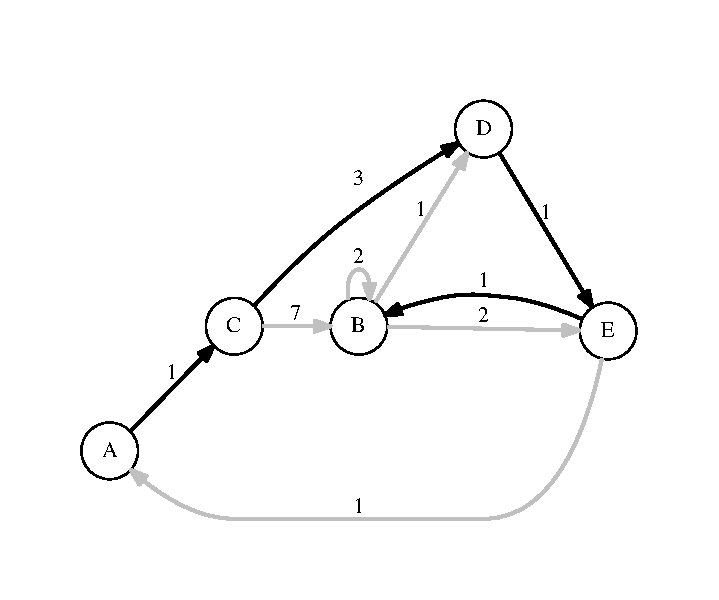
\includegraphics[width=1.\textwidth]{figuras/grafo-dijkstra} 
\caption{Aplicação do algoritmo de Dijkstra tendo o vértice "A" como origem. As arestas pintadas de preto correspondem a rota calculada a todos os demais vértices.}
\label{fig-dijkstra-algoritmo-grafo}
\end{figure}


\subsection{Garantia do algoritmo retorna o menor valor}
\label{sec-dijkstra-algoritmo-prova}
A prova será demonstrada em breve.

\section{Versões do Algoritmo implmentadas e suas Estrutura de Dados}
\label{sec-dijkstra-versoes}
Para este projeto de graduação, será implementada três versões do algoritmo de Dijkstra baseados em estruturas de dados diversas que implicam em tempos computacionais diferentes \cite{cormen2009introduction}.

As versões implementadas são o Dijkstra Canônico, Dijkstra Heap Binário (seção \ref{sec-dijkstra-versoes-heap}) e Dijkstra Heap de Fibonacci (seção \ref{sec-dijkstra-versoes-fibonacci}), todas baseadas em \citeonline{cormen2009introduction, drozdek2012data}.

Para a versão Dijkstra Canônico, o algoritmo utiliza de um vetor para armazenar as distâncias calculadas pelo algoritmo (assim como os seus vértices correspondetes, que neste caso é utilizado o próprio indíce do vetor armazenado), e a cada passo iterativo (conforme demonstrado pelo algoritmo na seção \ref{sec-dijkstra-algoritmo}), uma busca linear é realizada para determinar o vértice (fora do conjunto "toBeChecked") cuja a distância é menor dentre todas as outras. O tempo computacional para esse caso é $O(|V^{2}|)$ \cite{drozdek2012data}.

\subsection{Dijkstra Heap Binário (A revisar)}
\label{sec-dijkstra-versoes-heap}
Para esta implementação, será utilizada a estrutura de dados heap binária mínima como fila de prioridade. Heaps binária podem ser descritas como árvores binárias que possuem as seguintes propriedades \cite{drozdek2012data}:
\begin{enumerate}
 \item O valor de cada nodo não é maior do que os valores guardados em cada um de seus filhos.
 \item A árvore é perfeitamente balaceada, e as folhas no último nível estão todas mais a esquerda.
\end{enumerate}

Um exemplo de estrutura Heap Binário representada tanto como árvore como vetor pode ser visualizado nas figuras \ref{fig-dijkstra-heapbinario} e \ref{fig-dijkstra-heapvetor} respectivamente.

\begin{figure}[H]
\centering
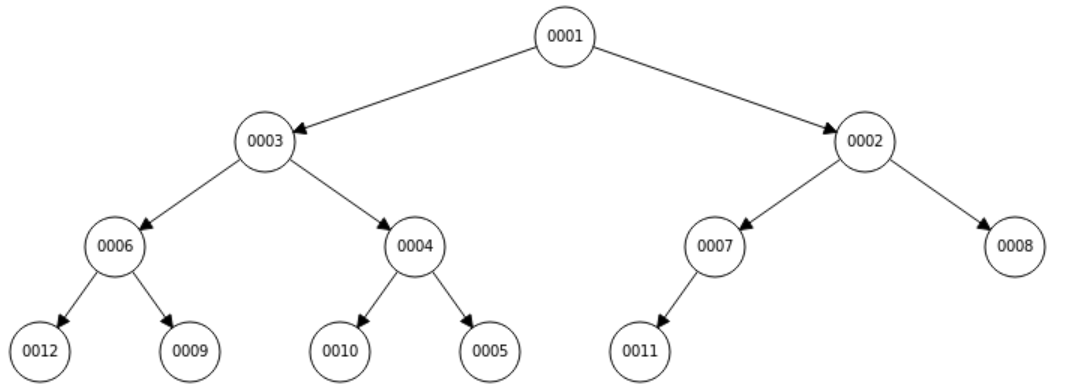
\includegraphics[width=.95\textwidth]{figuras/Heap} 
\caption{Exemplo de Heap Binário representado como árvore.}
\label{fig-dijkstra-heapbinario}
\end{figure}

\begin{figure}[H]
\centering
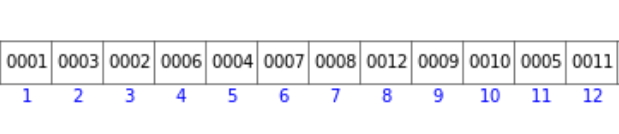
\includegraphics[width=.60\textwidth]{figuras/Heap-vetor}
\caption{Representação do Heap Binário da figura \ref{fig-dijkstra-heapbinario} como vetor.}
\label{fig-dijkstra-heapvetor}
\end{figure}

A vantagem de se usar essa estrutura de dados reside no fato de suas operações de inserção, extração de mínimo e reconstrução da heap possuirem tempo computacional de $O(\log n)$. Por consequência, o tempo computacional para este caso é de $O(|E| \log |V|)$ \cite{cormen2009introduction}.

\subsection{Dijkstra Heap de Fibonacci}
\label{sec-dijkstra-versoes-fibonacci}


\section{Experimentos Computacionais}
\label{sec-dijkstra-experimentos}
Para a realização dos experimentos computacionais será rodado instâncias de grafos que representam malhas rodoviárias reais. Todas elas descritas nas tabelas \ref{tbl-dijkstra-instancias} e \ref{tbl-dijkstra-configuracao}, e disponíveis no sítio eletrônico \url{http://www.dis.uniroma1.it/challenge9/download.shtml} (acesso em 28 de janeiro de 2017).
\begin{table}[H]
\caption{Instâncias a serem rodadas pelo algoritmo de Dijkstra em suas três versões.}
\label{tbl-dijkstra-instancias}
\centering
\begin{adjustbox}{max width=\textwidth}
\begin{tabular}{|c|c|}
\hline 
\textbf{Nome Instância} & \textbf{Descrição} \\ 
\hline 
USA-road-d.NY.gr & Representa a malha viária do estado de Nova Iorque, Estados Unidos \\ 
\hline 
USA-road-d.BAY.gr & Representa a malha viária da bahia de São Francisco, Califórnia, Estados Unidos \\ 
\hline 
USA-road-d.COL.gr & Representa a malha viária do estado do Colorado, Estados Unidos \\ 
\hline 
USA-road-d.FLA.gr & Representa a malha viária do estado da Flórida, Estados Unidos \\ 
\hline 
\end{tabular}
\end{adjustbox}
\end{table}

\begin{table}[H]
\caption{Configuração dos grafos correspondestes as malhas viárias descritas na tabela \ref{tbl-dijkstra-instancias}.}
\label{tbl-dijkstra-configuracao}
\centering
\begin{adjustbox}{max width=\textwidth}
\begin{tabular}{|c|c|c|}
\hline 
\textbf{Nome Instância} & \textbf{Número de Vértices |V|} & \textbf{Número de Arestas |E|} \\ 
\hline 
USA-road-d.NY.gr
 & 264.346
 & 733.846
 \\ 
\hline 
USA-road-d.BAY.gr
 & 321.270
 & 800.172
 \\ 
\hline 
USA-road-d.COL.gr
 & 435.666
 & 1.057.066
 \\ 
\hline 
USA-road-d.FLA.gr
 & 1.070.376
 & 2.712.798
 \\ 
\hline 
\end{tabular}
\end{adjustbox} 
\end{table}

\subsection{Resultados}
\label{sec-dijkstra-experimentos-resultados}


\section{Conclusões}
\label{sec-dijkstra-conclusoes}
Conforme apresentado por \citeonline{larkin2014back}.
% ==============================================================================
% TCC - Nome do Aluno
% Capítulo 3 - Especificação de Requisitos
% ==============================================================================
\chapter{Especificação de Requisitos}
\label{sec-requisitos}

Texto.

% ==============================================================================
% TCC - Nome do Aluno
% Capítulo 3 - Projeto Arquitetural e Implementação
% ==============================================================================
\chapter{Projeto Arquitetural e Implementação}
\label{sec-projeto}

Texto.

% ==============================================================================
% TCC - Nome do Aluno
% Capítulo 3 - Considerações Finais
% ==============================================================================
\chapter{Considerações Finais}
\label{sec-conclusoes}

Texto.




%%% Páginas finais do documento: bibliografia e anexos. %%%

% Finaliza a parte no bookmark do PDF para que se inicie o bookmark na raiz e adiciona espaço de parte no sumário.
\phantompart

% Marca o início dos elementos pós-textuais.
\postextual

% Referências bibliográficas
\bibliography{bibliografia}


% Apêndices.
\begin{apendicesenv}

% Imprime uma página indicando o início dos apêndices.
\partapendices

% (*) Incluir como apêndice a documentação técnica produzida durante o PG (especificação de requisitos,
% projeto arquitetural, etc.). Utilizar o exemplo \includepdf caso o documento seja produzido em outro
% editor de texto (Microsoft Word, LibreOffice Writer) e transformado em PDF. Utilizar o exemplo \include
% caso os documentos tenham sido também escritos em LaTeX.
% \includepdf[pages={1-}]{apendices/apendice01-requisitos.pdf}
% \includepdf[pages={1-}]{apendices/apendice02-projeto.pdf}
% \include{ap1-requisitos}
% \include{ap2-projeto}
\end{apendicesenv}


% Índice remissivo.
\phantompart
\printindex

% Fim do documento.
\end{document}
